
\begin{figure}
	\includegraphics[width=.9\linewidth]{../../output/figures/longclust/fig_traj_18_75_3333_nw_curt}
	\caption[Longitudinal clusters plot of of wealth over the lifetime]
	{Longitudinal clusters plot of  wealth over the lifetime} 
	\par \footnotesize \vspace{5pt}
	Notes:  The plot depicts average wealth for each group over the life-cycle. 
	Model fitted based on censored normal distribution specification and four clusters. 
	Fitted using the cubic  root  transformation of  gross wealth.
	Non-linear scale on vertical axis. 
	Percentages in graph legend show the cluster size of each group.
	\label{fig:trajplot}
\end{figure}

\begin{figure}
	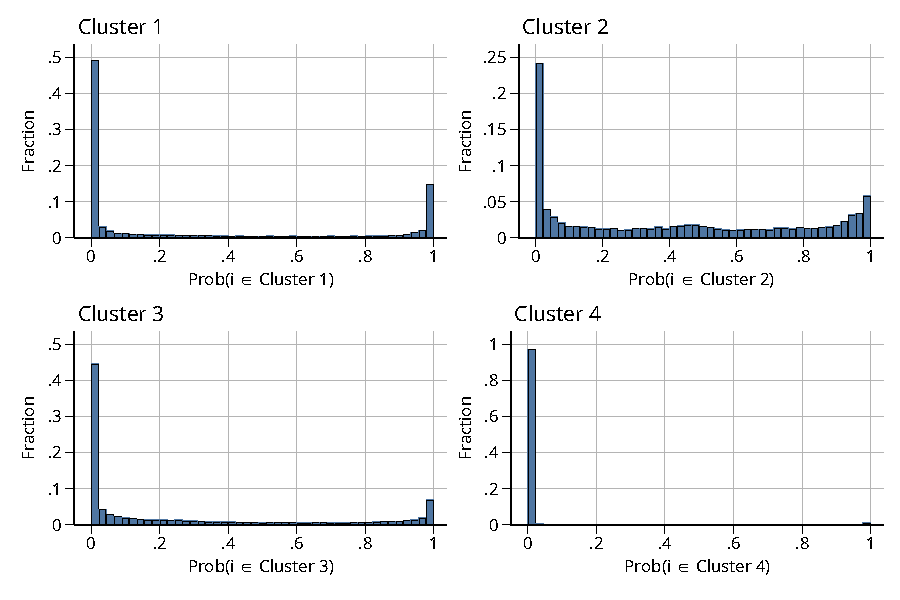
\includegraphics[width=.9\linewidth]{../../output/figures/longclust/fig_cluster_prob.pdf}
	\caption[Histograms of estimated probabilities of cluster classification]
	%	{Histograms of estimated probabilities ottttf cluster classification} 
	\par \footnotesize \vspace{5pt}
	Notes: The relatively high mass close to 0 and 1 indicates that the trajectories could be well separated.  Graphs indicate that belonging to clusters 1 and 4 are more distinct than 2 and 3, which show more mass in the range between 0 and 1. Wealth deflated by consumer price index from the German Federal Statistical Office (Destatis). 	 
	Note that the vertical axis do not share same scale across each cluster graph.
	\label{fig:trajplot}
\end{figure}